 \documentclass[letter,12pt]{article}
%
\usepackage[left=1in, top=1in, bottom=1in, right=1in]{geometry}

% packages 
\usepackage{latexsym,amssymb,amsmath,color}
%\usepackage{theorem}
\usepackage{graphicx}
%\usepackage[colorlinks=true]{hyperref}
%\hypersetup{urlcolor=blue, citecolor=red}
%\usepackage{algorithmic}
%\usepackage{algorithm}
\usepackage{cite}
\usepackage{verbatim}
\usepackage[table]{xcolor}

% -------------- macros
\newcommand{\p}{\partial}
\def\Cb{\overline{C}}

\newcommand{\R}{\mathbb{R}}
\newcommand{\N}{\mathbb{N}}
\newcommand{\cov}{\mathrm{cov}}
\newcommand{\iid}{\stackrel{iid}{\sim}}
\newcommand{\F}{\mathcal{F}}%
\newcommand{\be}{\begin{equation}}
\newcommand{\ee}{\end{equation}}
\newcommand{\bea}{\begin{eqnarray}}
\newcommand{\eea}{\end{eqnarray}}
%\newcommand{\p}{\partial}
\newcommand{\ttt}{\tilde}
%
\def\Wb{\overline{W}}
\def\td{\tilde \delta}
\def\tL{\tilde L}
\def\tU{\tilde U}
\def\tt{\tilde t}
\def\Vector#1{\mbox{\boldmath $#1$}}
\def\vH{{\Vector H}}
\def\vx{{\Vector x}}
\def\vy{{\Vector y}}
\def\vz{{\Vector z}}
\def\vj{{\Vector j}}
\def\vk{{\Vector k}}
\def\vt{{\Vector t}}
\def\ve{{\Vector e}}
\def\vb{{\Vector b}}
\def\vg{{\Vector g}}
\def\vn{{\Vector n}}
\def\vp{{\Vector p}}
\def\vr{{\Vector r}}
\def\vS{{\Vector S}}
\def\vV{{\Vector V}}
\def\vY{{\Vector Y}}
\def\vX{{\Vector X}}
\def\vv{{\Vector v}}
\def\vu{{\Vector u}}
\def\vQ{{\Vector Q}}
\def\vZ{{\Vector Z}}
\def\vN{{\Vector N}}
\def\vF{{\Vector F}}
\def\vC{{\Vector C}}
\def\vq{{\Vector q}}
\def\vom{{\Vector \omega}}
\def\vtau{{\Vector \tau}}
\def\F{{\rm\bf F}}
\def\sech{{\rm sech}}
\def\funnyzeta{\varsigma}
\def\tQ{\stackrel{\ldots}{Q}}
%
\def\Re{{\rm Re}}
\def\Sc{{\rm Sc}}
\def\Pe{{\rm Pe}}
\def\Pr{{\rm Pr}}
\def\Da{{\rm Da}}
\def\rf{{\rm ref}}
\def\eps{{\varepsilon}}
\def\ep{\epsilon'}
\def\O{{\rm O}}
\def\1{{\rm 1}}
\def\so{^{\rm (0)}}
\def\s1{^{\rm (1)}}
\def\d{{\rm d}}
\def\ttm{^{{\rm ttm}}}
\def\img{^{\rm im}}
\def\si{^{\rm si}}
%
\def\ol{\overline}
%
\def\tn{^{n}}
\def\tnm{^{n-1}}
\def\new#1{{\bf #1}}
%\def\new#1{{#1}}

\renewcommand{\L}{\mathcal{L}}
\newcommand{\Q}{\mathcal{Q}}
\newcommand{\U}{\mathcal{U}}
\newcommand{\G}{\mathcal{N}}
\newcommand{\V}{\mathcal{V}}
\renewcommand{\P}{\mathrm{P}}
\newcommand{\B}{\mathcal{B}}
\renewcommand{\vec}[1]{{\mathchoice
                     {\mbox{\boldmath$\displaystyle{#1}$}}
                     {\mbox{\boldmath$\textstyle{#1}$}}
                     {\mbox{\boldmath$\scriptstyle{#1}$}}
                     {\mbox{\boldmath$\scriptscriptstyle{#1}$}}}}
\newcommand{\var}[1]{{\mathrm{Var}}\left( {#1} \right)}
\newcommand{\normim}[1]{\left\| {#1} \right\|_{\scriptscriptstyle L^{2}(\Omega^{*})}}
\newcommand{\avemu}[1]{\mathrm{E}\left({#1}\right)}
\newcommand{\ave}[1]{\left\langle {#1} \right\rangle}
\newcommand{\prob}[1]{\mathrm{Prob}\left\{ {#1} \right\}}
\newcommand{\ind}[1]{\mathrm{\chi}_{\scriptscriptstyle {#1} }}
\newcommand{\NISP}{\mathcal{S}}
\newcommand{\xxi}{\vec{\xi}}
\newcommand{\ip}[2]{\left( {#1}, {#2} \right)}
\newcommand{\ipmu}[2]{\left( {#1}, {#2} \right)_\mu}
\newcommand{\norm}[1]{\left\| {#1} \right\|_{\scriptscriptstyle L^{2}(\Omega)}}
\newcommand{\normone}[1]{\left\| {#1} \right\|_{\scriptscriptstyle 1}}
\newcommand{\pard}[2]{\frac{\partial{#1}}{\partial{#2}}}
%
%\newcommand{\be}{\begin{equation}}
%\newcommand{\ee}{\end{equation}}
%\newcommand{\bea}{\begin{eqnarray}}
%\newcommand{\eea}{\end{eqnarray}}
%\newcommand{\p}{\partial}
%\newcommand{\ttt}{\tilde}
%
\def\Wb{\overline{W}}
\def\td{\tilde \delta}
\def\tL{\tilde L}
\def\tU{\tilde U}
\def\tt{\tilde t}
\def\Vector#1{\mbox{\boldmath $#1$}}
\def\vH{{\Vector H}}
\def\vx{{\Vector x}}
\def\vy{{\Vector y}}
\def\vz{{\Vector z}}
\def\vj{{\Vector j}}
\def\vk{{\Vector k}}
\def\vt{{\Vector t}}
\def\ve{{\Vector e}}
\def\vb{{\Vector b}}
\def\vg{{\Vector g}}
\def\vn{{\Vector n}}
\def\vp{{\Vector p}}
\def\vr{{\Vector r}}
\def\vS{{\Vector S}}
\def\vV{{\Vector V}}
\def\vY{{\Vector Y}}
\def\vX{{\Vector X}}
\def\vv{{\Vector v}}
\def\vu{{\Vector u}}
\def\vQ{{\Vector Q}}
\def\vZ{{\Vector Z}}
\def\vN{{\Vector N}}
\def\vF{{\Vector F}}
\def\vC{{\Vector C}}
\def\vq{{\Vector q}}
\def\vom{{\Vector \omega}}
\def\vtau{{\Vector \tau}}
\def\F{{\rm\bf F}}
\def\sech{{\rm sech}}
\def\funnyzeta{\varsigma}
\def\tQ{\stackrel{\ldots}{Q}}
%
\def\Re{{\rm Re}}
\def\Sc{{\rm Sc}}
\def\Pe{{\rm Pe}}
\def\Pr{{\rm Pr}}
\def\Da{{\rm Da}}
\def\rf{{\rm ref}}
\def\eps{{\varepsilon}}
\def\ep{\epsilon'}
\def\O{{\rm O}}
\def\1{{\rm 1}}
\def\so{^{\rm (0)}}
\def\s1{^{\rm (1)}}
\def\d{{\rm d}}
\def\ttm{^{{\rm ttm}}}
\def\img{^{\rm im}}
\def\si{^{\rm si}}
%
\def\ol{\overline}
%
\def\tn{^{n}}
\def\tnm{^{n-1}}
\def\new#1{{\bf #1}}
\newcommand{\todo}[1]{\scshape\color{red}{#1}}
%
 \def\ol{\overline}
 \def\no{\noindent}
 \def\qd{\dot{Q}}
% ----------------- end macros

\usepackage[table]{xcolor}
\usepackage{relsize}
\usepackage{bm}
\usepackage{mathrsfs}

 \def\ol{\overline}
 \def\no{\noindent}
 \def\qd{\dot{Q}}

%%%%%%%FLOW DIAGRAM%%%%%%%%%%
\usepackage[latin1]{inputenc}
\usepackage{tikz}
%\usepackage[table]{xcolor}
\usetikzlibrary{shapes,arrows}
% Define block styles
\tikzstyle{decision} = [diamond, draw, fill=blue!20, 
   text width=5.0em, text badly centered, node distance=3cm, inner sep=0pt]
\tikzstyle{block} = [rectangle, draw, fill=cyan!20, 
   text width=9.0em, text centered, rounded corners]
\tikzstyle{line} = [draw, -latex']
\tikzstyle{cloud} = [draw, ellipse,fill=red!20, node distance=3cm,
   minimum height=2em]
%%%%%%%%%%%%%%%%%%%%%%%%%%

%-------------------------------------------------------------------
\begin{document}

\begin{center}
\textsc{
Derivative-based global sensitivity approach to efficient surrogate modelling
with Polynomial Chaos
}

\bigskip 
\bigskip 

Manav Vohra$^{1}$, Alen Alexanderian$^{2}$, Cosmin Safta$^{3}$, Sankaran Mahadevan$^{1}$

\bigskip
\bigskip

\normalsize
$^1$Department of Civil and Environmental Engineering\\
Vanderbilt University\\
Nashville, TN 37235\\

\bigskip

$^2$Department of Mathematics\\
North Carolina State University\\
Raleigh, NC 27695\\

\bigskip

$^3$Sandia National Laboratories\\
Livermore, CA 94550\\

\end{center}

\vspace{6cm}

\begin{tabbing}
Corresponding Author: \hspace{5mm} \= Sankaran Mahadevan\\
       \>  Department of Civil and Environmental Engineering\\
       \>  Vanderbilt University\\
       \>  272 Jacobs Hall, VU Mailbox: PMB 351831 \\
       \>  Nashville, TN 37235 \\
       \> \\
Phone: \> (615) 322-3040 \\
Fax:   \> (615) 343-3773 \\
Email: \>  sankaran.mahadevan@vanderbilt.edu   \\
\\
Submitted to: \> \textit{Reliability Engineering and System Safety} \\
\>  May 2018\\

\bigskip
\end{tabbing}

\clearpage



\tableofcontents

\section{Introduction}
\label{sec:intro}

%\begin{enumerate}
%\item Need for efficient Surrogates - especially for complex models to enable forward UQ, 
%sensitivity studies, calibration, and experimental design (Include citations).
%\item Computational Hurdles: Polynomial Chaos and GP can be computationally 
%intractable and suffer from the curse of dimensionality (Include plots for PCE
%to motivate dimension reduction with citations for both PCE and GP).
%\item Sensitivity analyis - a potent tool for dimension reduction. However, SA can be
%computationally prohibitive. In fact, there are studies demonstrating the use of 
%surrogates to reduce costs associated with SA (include citations). 
%\item DGSM - brief introduction and citations. 
%\item Key contributions of the paper: 1) Methodology that exploits DGSM to reduce the
%dimensionality of the problem and thus enables efficient construction of surrogates.
%2) Application of the proposed methodology to investigate relative importance of
%parameters in the stillinger-weber potential, commonly used for studying phonon transport in silicon. Further, construct a reasonably accurate PC surrogate in the reduced 
%space and demonstrate computational advantage of this approach. .
%\end{enumerate}

The emerging field of uncertainty quantification (UQ) aims at methodologies for 
incorporating, characterizing, quantifying, propagating, and reducing the 
uncertainties associated with predictive models and simulations. For situations
involving complex physical models and compute-intensive simulations, an
efficient approach to construction of model surrogates is sought to enable UQ
in a tractable manner. Polynomial chaos expansion 
(PCE)~\cite{Xiu:2002,Ghanem:2003,Eldred:2008,Olivier:2010} and 
Gaussian Process (GP)~\cite{Rasmussen:2004} or Kriging~\cite{Stein:2012} are
among the most commonly used surrogates for scientific applications. However,
both approaches quickly become prohibitive when the set of uncertain model
inputs and parameters is large-dimensional. Specifically, in the case of a PCE,
a $d$-dimensional polynomial basis with a total order of truncation, $p$ 
requires model realizations at $(p+1)^d$ quadrature nodes to estimate the PC
coefficients using a fully-tensorized Gauss quadrature. This trend is 
illustrated below in Figure~\ref{fig:curse}.

\begin{figure}[htbp]
 \begin{center}
  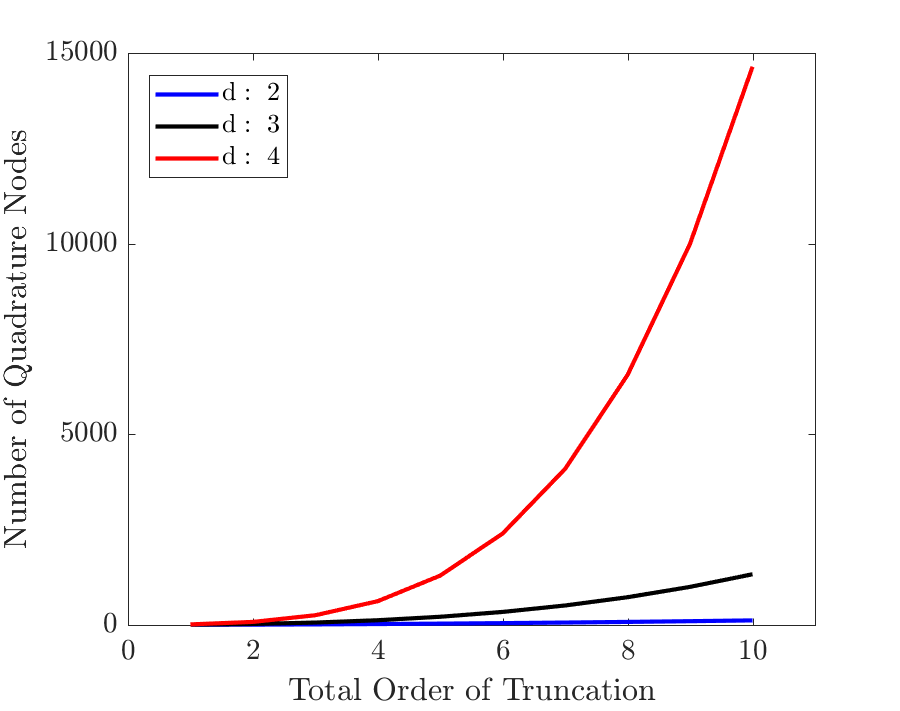
\includegraphics[width=0.70\textwidth]{./Figures/quad_comp}
\caption{Number of fully-tensorized Gauss quadrature nodes ($(p+1)^d$) is plotted against PCE total order truncation, $p$ for $d$ = 2,3, and 4.}
\label{fig:curse}
\end{center}
\end{figure}






\section{Background}
\label{sec:bg}

In this section, we introduce the notations used in the rest of
the article, and present the requisite background material on 
derivative-based global sensitivity measures and surrogate modeling 
using polynomial chaos expansion.




\subsection{Derivative-based global sensitivity analysis}  

Let $\GG$ be a mathematical model that is a function of $\Np$ uncertain 
parameters, $\theta_1, \theta_2, \ldots, \theta_\Np$. The goal of sensitivity analysis
is measuring the influence of each component of the parameter vector 
$\bm{\theta}$ on the model output. 
In the present work, we consider the case where the input parameters are statistically 
independent. 

Derivative-based global sensitivity analysis (DGSA) is performed by 
computing derivative based global sensitivity measures (DGSMs)~\cite{Sobol:2009} 
for each uncertain parameter in the model. 
Specifically, we consider the following DGSMs, 
\be
\mu_i = 
\mathbb{E}\left[\left(\frac{\partial \GG(\bm{\bm{\theta}})}{\partial \theta_i}\right)^{2}\right], \quad i = 1, \ldots, \Np.
\label{eq:mu}
\ee
Here $\mathbb{E}$ denotes expectation over the uncertain parameters.
Notice that this formulation assumes that the function $\GG$ is differentiable
with respect to $\theta_i$, $i = 1, \ldots, \Np$, almost surely.

If an analytic expression for $\GG$ is available the derivative in the above
expression can be computed directly. In applications, however, $\GG$ is often
defined in terms of a solution of a mathematical model. In some cases, 
one has access to appropriate adjoint solvers that enable efficient
adjoint-based gradient computations. In the present work, we consider
a generic computational model and only assume that the model
output depends differentiablly to the parameter $\bm{\theta}$. Thus, 
we consider finite-difference gradient computation: 
\be
\frac{\partial \GG(\bm{\theta})}{\partial \theta_i} 
\approx
\frac{\GG(\theta_1,\ldots,\theta_{i-1},
\theta_i+\Delta\theta_i,
\theta_{i+1},\ldots,\theta_d) - 
\GG(\bm{\theta})}{\Delta\theta_i}, \quad i = 1, \ldots, \Np. 
\label{eq:partial}
\ee
Then,~\eqref{eq:mu} can be evaluated by Monte Carlo sampling in
the uncertain parameter space. 
The total number of model realizations or function evaluations
needed to
compute $\mu_i$ for a function $G$ of $\Np$ random inputs and using $N$ samples is
therefore, $N\times(\Np+1)$. 
%The derivative in Eq.~\ref{eq:partial} could be evaluated
%analytically in case the functional dependence of $\GG$ and $\theta_i$
%is known. 
%Note that the perturbation $\Delta\theta_i^{*}$ is extremely small 
%compared to the uncertainty in $\theta_i$ which leads to a significant improvement
%over the `elementary effect' of a parameter, estimated in the Morris method~\cite{Morris:1991}
%using large increments.  
It is noted by many authors~[REFS], and also observed
in the numerical experiments in the present work, that a modest Monte Carlo
sample size is often sufficient for computing~\eqref{eq:mu} with reasonable
accuracy.

Consider the total 
Sobol' sensitivity index~\cite{Sobol:2001},
\be
\mathcal{T}(\theta_i) = 1 - 
\frac{\mathbb{V}[\mathbb{E}(\GG|\bm{\theta}_{\sim i})]}{\mathbb{V}(\GG)},
\label{eq:total}
\ee
where $\bm{\theta}_{\sim i}$ is the random vector $\bm\theta$ with $i$th component removed, 
and $\mathbb{V}$ denotes the variance. The total Sobol' index quantifies the total contribution 
of $\theta_i$ to variance of the model $\GG$. Components of $\bm\theta$ with small 
total Sobol' index can be considered inessential and can be fixed at nominal values. However, 
computing the total Sobol' index is a computationally expensive task for expensive-to-evaluate 
models with large number of uncertain parameters. Fortunately, 
for parameters with continuous distributions, an upper bound on $\mathcal{T}_i$  
can be expressed in terms of $\mu_i$, the Poincar\'e constant ($\mathcal{C}_i$) and the total 
variance of the model output ($\mathbb{V}(\GG)$)~\cite{Lamboni:2013}:
\be
\mathcal{T}(\theta_i) \leq \frac{\mathcal{C}_i\mu_i}{\mathbb{V}(\GG)}~(\propto \widehat{\mathcal{C}_i\mu_i})
\label{eq:bound}
\ee

\noindent The upper bound in the above inequality is proportional to the product of $\mathcal{C}_i$
and $\mu_i$. However, for the purpose of parameter screening as discussed later in
Section~\ref{sec:method}, we consider a normalized product, $\widehat{\mathcal{C}_i\mu_i}$:

\be
\widehat{\mathcal{C}_i\mu_i} = \frac{\mathcal{C}_i\mu_i}{\sum_i \mathcal{C}_i\mu_i}
\label{eq:cmu}
\ee

\noindent The Poincar\'e constant, $\mathcal{C}_i$ is specific to the probability distribution of $\theta_i$.
Table~\ref{tab:poincare} provides its value in the case of uniform and normal
distributions.
\bigskip

\begin{table}[htbp]
\renewcommand*{\arraystretch}{1.2}
\begin{center}
\begin{tabular}{|c|c|}
\hline
Distribution & $\mathcal{C}_i$ \\ \hline \hline 
Uniform, $\mathcal{U}[a, b]$ & $(b-a)^{2}/\pi^2$ \\ 
Normal, $\mathcal{N}(\mu,\sigma^2)$ & $\sigma^2$ \\ 
\hline
\end{tabular}
\end{center}

\caption{Poincare constant for the case of uniformly and normally distributed random
parameters~\cite{Roustant:2014}.}
\label{tab:poincare}
\end{table}

\subsection{Polynomial chaos expansion}

We consider models with $\Np$ random inputs, 
$\theta_1, \ldots, \theta_\Np$ that are modeled
as statistically independent random variables. The 
variables $\theta_i$ will take in physically meaningful
ranges; it is common to parameterize input uncertainties
with canonical random variables $\xi_1, \ldots, \xi_\Np$,
which can be then shifted and scaled to obtain the corresponding $\theta_i's$.
Typical choices for distribution of $\xi_i$ include standard normal 
and uniform distribution on the interval $[-1, 1]$.
Let 
\[
   \bm{f}(\bm{x}) = \prod_{i=1}^\Np f_i(x_i), \quad \bm{x} \in \mathbb{R}^\Np
\]
where $f_i$ are probability density functions of $\xi_i$, $i = 1, \ldots, \Np$.
We consider a square integrable random variable $\GG:\R^\Np \to \R$; 
that is,
\[
\int_{\mathcal{D}} \GG(\bm{\xi})^2 \, \bm{f}(\bm{\xi})d\bm{\xi} < \infty,
\]
where $\mathcal{D}$ is the support of the distribution law of the random vector
$\bm{\xi}$. 


% for representing the
%dependence of a random observable ($\GG$) on independent uncertain or
%stochastic model parameters ($\bm{\theta}$).  Considering a joint probability
%distribution of the components of ($\bm{\theta}$) as
%$\mathbb{P}(\bm{\theta})$, the following condition is imposed on
%$\GG$:
%\be
%\mathbb{E}[\GG^2] = \int_{\mathcal{D}_{\bm{\theta}}} \GG^2 \mathbb{P}(\bm{\theta}) 
%d\bm{\theta} < \infty
%\ee

%\noindent where $\mathcal{D}_{\bm{\theta}}$ is the domain of the input parameter space. 

As mentioned in Section~\ref{sec:intro}, the 
polynomial chaos expansion
(PCE) is a commonly used tool for surrogate modeling. 
The PCE of
$\GG$ is a mean-square 
convergent series expansion~\cite{Xiu:2002,Ghanem:2003,Olivier:2010} of the form:
\be
\GG(\bm\xi) = \sum_{k=0}^\infty c_k\Psi_k(\bm{\xi}),
\ee
where $\Psi_k$'s form a multivariate orthogonal polynomial
basis---orthogonal with respect to the joint probability distribution of $\bm{\xi}$.
%
In practice, a truncated expansion is used.  Moreover, in applications, $\GG$
is a mathematical model of interest that takes a parameter vector $\bm{\theta}$
(with components in physically meaningful ranges) as input. Therefore, we 
write the truncated PC representation of a model $\GG$ as follows:
\be 
\GG(\bm\theta) \approx \GG^{\mbox{\tiny PC}}(\bm\theta) := \sum_{k=0}^{\Npc}
c_k\Psi_k (\bm\xi(\bm\theta)), 
\ee
where $\bm\xi(\bm\theta)$ is found by a simple linear transformation.

Computational strategies available for estimating the PC coefficients
($c_k$'s) typically involve techniques based on projection or regression.
Projection-based methods consider the orthogonal projection of 
$\GG$ on the PC basis $\{\Psi_k\}_{k=0}^\Npc$ and compute
the resulting expansion coefficients via quadrature~\cite{Olivier:2010}.
%on numerical quadrature for estimating the
%following expectation:
%\be
%\bm{c} = \mathbb{E}[\Psi_\alpha(\bm{\xi})\cdot\GG^{\mbox{\tiny{M}}}]
%\approx
%\sum_{i=1}^{N} \GG^{\mbox{\tiny{M}}}(\bm{\theta}^{(i)})w^{(i)}\Psi_\alpha(\bm{\xi}^{(i)})
%\ee
%\noindent where $w^{(i)}$ denotes the weight associated with the quadrature node $i$. 
Regression-based methods such as least angle regression (LAR)~\cite{Efron:2004}, and least absolute shrinkage
and selection operator (LASSO)~\cite{Tibshirani:1996} aim to construct a sparse PCE~\cite{Blatman:2008}
by solving a regularized optimization problem. Specifically in the case of LAR, a penalty term comprising the L-1
norm of the PC coefficients is used:

\be
\hat{\bm{c}} = \mbox{argmin}~\mathbb{E}_{\bm\theta}
\left[\left(\sum_{k=0}^\Npc c_k \Psi_k(\bm\xi(\bm\theta)) -
\GG(\bm{\theta})\right)^{2}\right]  + \lambda\normone{\bm{c}}
\label{eq:reg}
\ee
where $\normone{\bm{c}}$ = $\sum_{k=0}^\Npc |c_k |$.
The regularization term forces the minimization towards sparse coefficient vectors resulting
in sparse PC representations.
In this work, we construct sparse PCEs with LAR using UQLab~\cite{Marelli:2014},
a general purpose uncertainty quantification software developed at ETH Zurich.
% in Switzerland.




















\section{Method}

\section{Motivating examples}
\subsection{Borehole: Screening, Convergence, Verification}
\subsection{Semilinear elliptic PDE: Screening, Convergence, Verification}
\subsection{Nonlinear Oscillator: Screening, Convergence, Verification}

\section{Application: Phonon Transport in a Si bar}

Seven uncertain parameters; well-established nominal values exist;
\[
   \theta_i \sim U(\bar\theta_i - \epsilon_i, \bar\theta_i + \epsilon_i), 
   \quad \epsilon_i = 0.1 \bar\theta_i. 
\]
\begin{enumerate}
\item Include all details pertaining to the MD simulation: system, simulation, 
ensembles, etc. 
\item Results
\end{enumerate}

\section{Discussion}
\begin{enumerate}
\item Methodology is agnostic to the choice of surrogate.
\item As required for a PCE, the uncertain parameters need not be independent. 
\item Strategy depends on the application - methodology could be implemented 
sequentially or adaptively. 
\end{enumerate}


\end{document}
